\chapter{Measurement Results}
\label{ch_results}

A summary of the measurement results can be found in Appendix \ref{ap_measurements}, and the detailed data is in the repository \hyperlink{https://github.com/smiths/AIMSS}{https://github.com/smiths/AIMSS}.

All of the 29 software packages that we measured are OSS with functions of displaying medical images. The initial release dates of these packages are between the years 1998 and 2018. We considered 2 of them as ``dead'' projects since they had the latest updates more than 18 months earlier than the time of measuring, but both had updates after 2017.

We found out that at least 8 of the projects received funding for at least a certain period, but we were not sure about the rest of them due to limited information. 

After analyzing the repositories and official websites of the projects, we found out that the number of contributors for a project varied between 1 to roughly 100. We considered anyone who made at least one accepted commit to the source code as a contributor, so it does not mean that any development teams had long-term members as many as 100. Many of these projects received change requests and code from the community, such as pull requests and git commits on GitHub. At least 27 of the software projects had code commits from more than a single developer, and as far as we could find out, at least 13 of them had no less than 10 contributors.

According to our measurements, 27 out of the 29 packages supported multiple operating systems, and 25 of them could work on all three Windows, macOS, and Linux systems. However, there was a significant difference in the philosophy to achieve cross-platform compatibility. The majority of the 27 were desktop software products built for each operating system separately. On the other hand, 5 were web applications, which made them naturally platform-independent and compatible with almost all operating systems with compatible browsers. There are certain advantages and disadvantages to developing either a native or a browser-based application, and some of the details can be found from the interview answers in Section \ref{ch_interviews}.

Most of the projects used more than one programming language, including a primary language that the developers used the most. The most popular primary language was C++, chosen by 11 projects, and another 3 teams selected C. The second most used one was JavaScript, with 6 projects using it as the primary language. 4 of the projects chose Java, and 3 selected Python.

\section{Overall Scores}

As described in Section \ref{sec_AHP}, for our AHP measurements, there are 9 criteria which are the 9 software qualities and 29 software packages as the alternatives. We decided to make all 9 qualities equally important, so the score of each quality affects the overall scores on the same scale.

Figure \ref{fg_overall_scores} shows the overall scores of all 29 software packages in descending order. Since we produced the scores from the AHP process, the total sum of the 29 scores is precisely 1.

\begin{figure}[H]
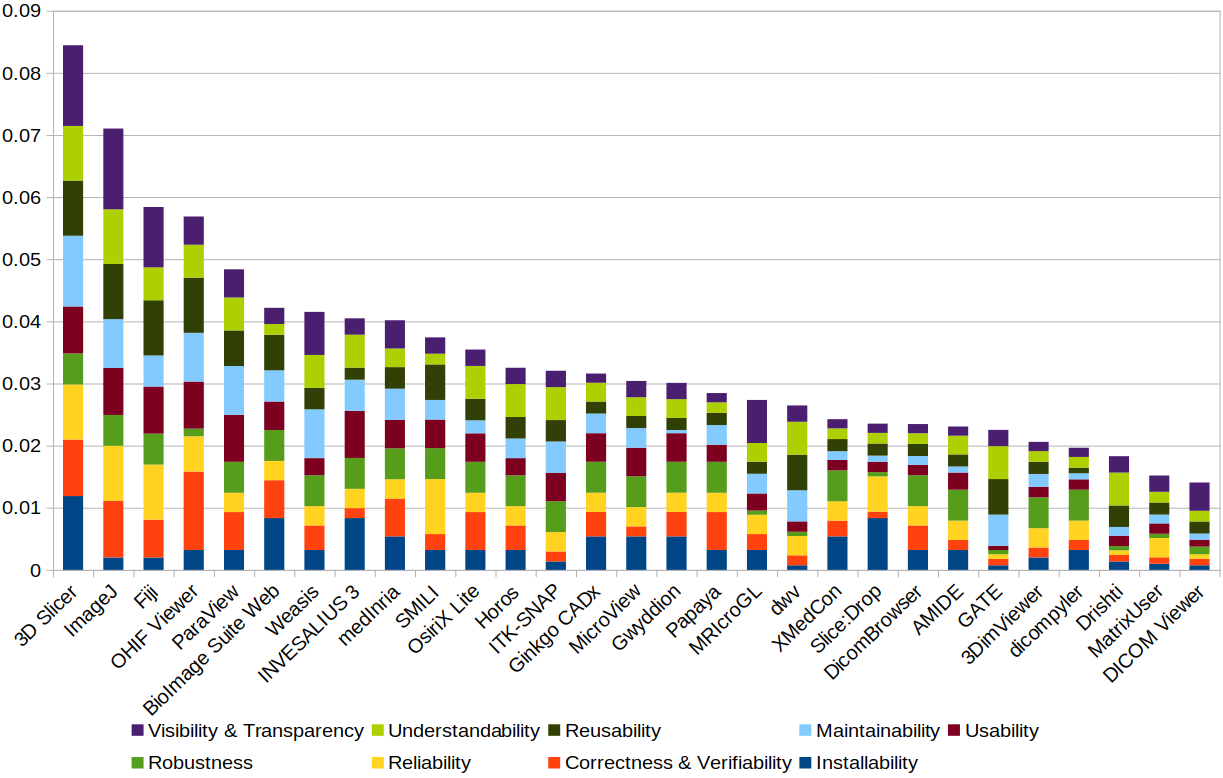
\includegraphics[scale=0.35]{figures/overall_scores.png}
\caption{Overall AHP scores for all 9 software qualities}
\label{fg_overall_scores}
\end{figure}

The top two software products had higher scores in each criterion. For example, \textit{3D Slicer} \cite{Kikinis2014} ranked at the first or second place for 8 of the 9 qualities; \textit{ImageJ} \cite{Rueden2017} was within the top three products for 7 qualities. There were 3 software packages that we
could not install or build correctly. Among them, \textit{DICOM Viewer} \cite{Afsar2021} was the only one that did not have an online test version, so that we could not finish all measurements for it. Consequently, we might underestimate its score.

\section{Installability}
\label{sec_result_installability}
When measuring the \textit{installability}, we checked the existence and quality of installation instructions. The user experience was also an important factor, such as the ease to follow the instructions, number of steps, automation tools, and the prerequisite steps for the installation. If any problem interrupted the process of installation or uninstallation, we gave a lower score to this quality. We also recorded the operating system for the installation test and whether we could verify the installation.

Figure \ref{fg_installability_scores} lists the scores of \textit{installability}, with a total sum of 1.

\begin{figure}[H]
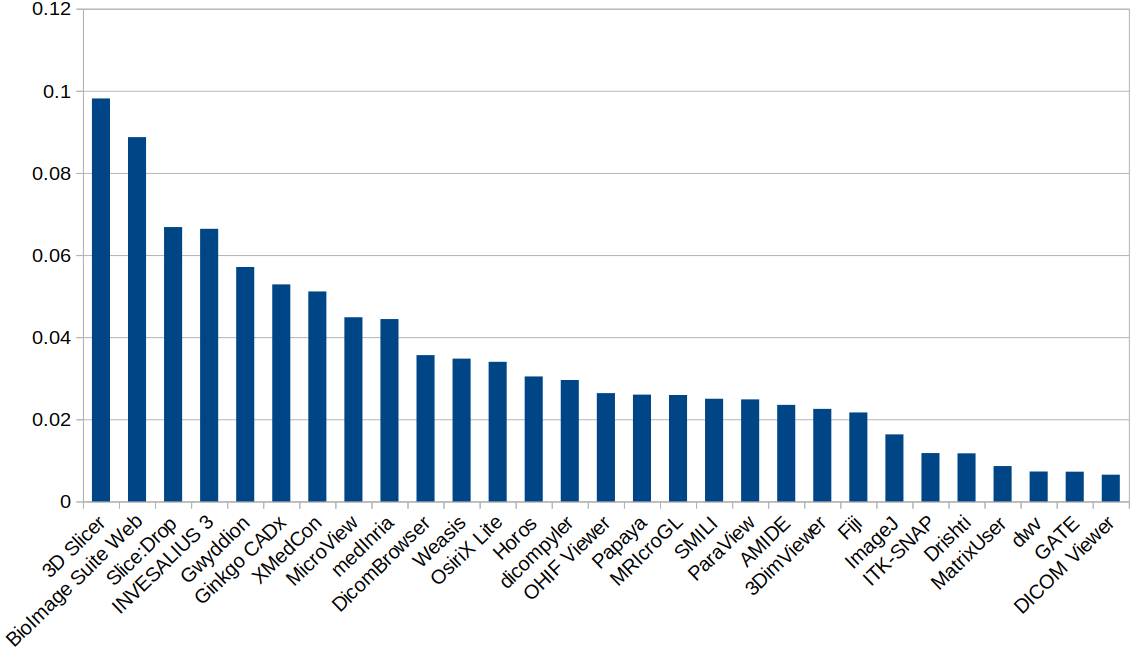
\includegraphics[scale=0.38]{figures/installability_scores.png}
\caption{AHP installability scores}
\label{fg_installability_scores}
\end{figure}

The projects with higher scores had easy-to-follow installation instructions, and the installation processes were automated, fast, and frustration-free, with all dependencies automatically added. There were also no errors during the installation and uninstallation steps.

The ones with the lowest scores often showed severe problems. We could not install some of them due to some issues that we could not solve. We spent a reasonable amount of time on these problems, then considered them major obstacles for normal users if we still did not figure out any solutions. For example, we needed to build some software from the source code, and we failed the building for two of them following the instructions. Furthermore, \textit{DICOM Viewer} depended on a cloud platform, and we could not successfully install the dependency. We suspect that only a part of the users faced the same problems, and given a lot of time, we might be able to find solutions. However, the difficulties greatly impacted the installation experiences, and we graded these software packages with lower scores.

Although we could not locally build two software packages, there were deployed online versions for them. With that, we finished all the measurements for them.

\section{Correctness \& Verifiability}

For \textit{correctness}, we checked the projects to identify the techniques to ensure this quality, such as literate programming, automated testing, symbolic execution, model checking, unit tests, etc. We also examined that whether the projects used continuous integration. As for \textit{verifiability}, we went through the documents of the project to check the requirements specifications, theory manuals, and getting started tutorial. If a getting started tutorial existed and provided expected results, we followed it and checked if the outputs match.

The scores of \textit{correctness \& verifiability} are shown in Figure \ref{fg_correctness_erifiability_scores}. Generally speaking, the packages with higher scores adopted more techniques to improve \textit{correctness}, and had better documents for us to verify it.

\begin{figure}[H]
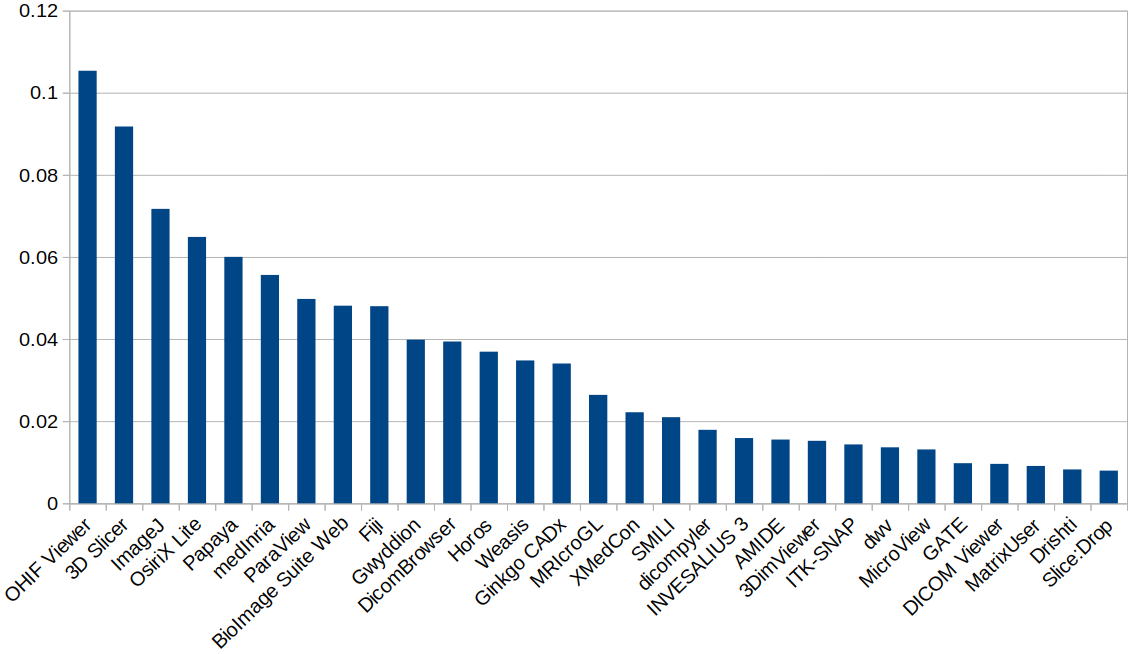
\includegraphics[scale=0.38]{figures/correctness_verifiability_scores.png}
\caption{AHP correctness \& verifiability scores}
\label{fg_correctness_erifiability_scores}
\end{figure}

After examining the source code, we could not find any evidence of unit testing in more than half of the projects. Unit testing benefits most parts of the software's life cycle, such as designing, coding, debugging, and optimization \cite{Hamill2004}. It can reveal the bugs at an earlier stage of the development process, and the absence of unit testing may cause worse \textit{correctness \& verifiability}. We also could not identify the requirements specifications or theory manuals for most of the projects. It seems that even for some projects with well-organized documents, requirements specifications and theory manuals were still missing.

\section{Surface Reliability}
For \textit{Surface Reliability}, we checked that whether the software broke during the installation and tutorial, whether there were descriptive error messages, and if we could recover the process after the errors.

As described in Section \ref{sec_result_installability}, we could not build two software packages, however, since there were online versions of them, which might be proof that successful deployments were possible. So the failure of installation did not affect their scores in \textit{Surface Reliability}. Figure \ref{fg_reliability_scores} shows the AHP results.

\begin{figure}[H]
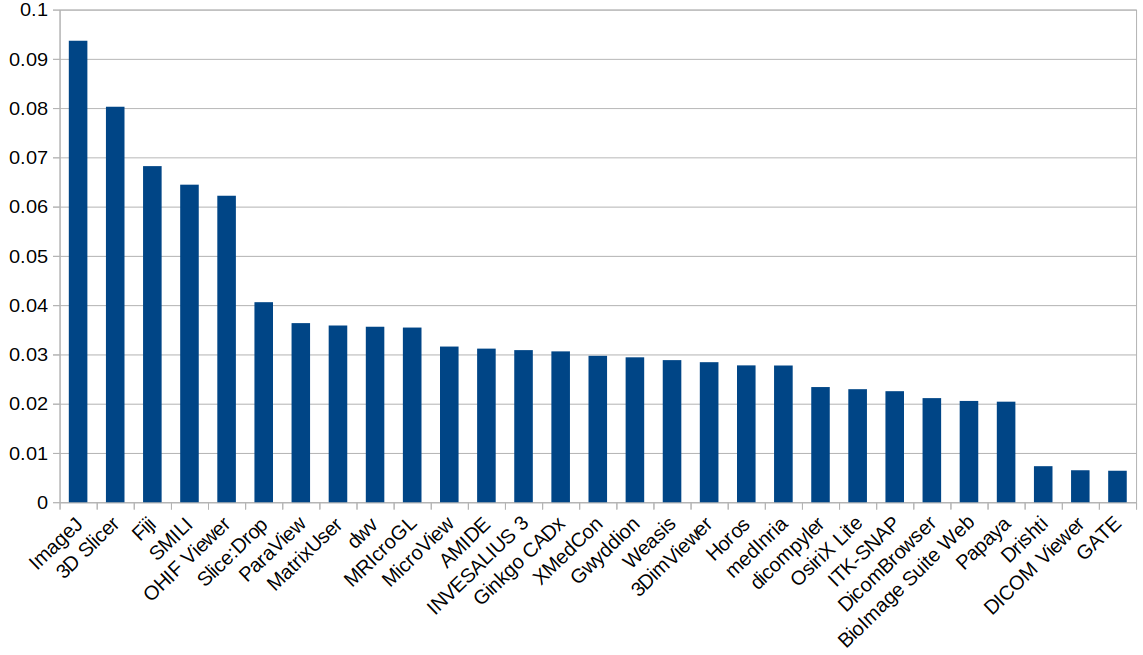
\includegraphics[scale=0.38]{figures/reliability_scores.png}
\caption{AHP surface reliability scores}
\label{fg_reliability_scores}
\end{figure}

For the software with the lowest scores, \textit{Drishti} \cite{Limaye2012} and \textit{GATE} \cite{Jan2004} crashed during our operations, and we might underestimated the score of \textit{DICOM Viewer} since we could not install or test it.

\section{Surface Robustness}

To test \textit{Surface Robustness}, we checked that how the software handle unexpected/unanticipated input. Since all 29 MI software packages had functions to load image files, we prepared broken image files for the software to open. For example, a text file (.txt) with a modified extension name (.dcm) can be used as an unexpected/unanticipated input. We first tried to load a few correct input files with the software to ensure the function was working correctly, then with the unexpected/unanticipated ones. Figure \ref{fg_robustness_scores} presents the scores.

\begin{figure}[H]
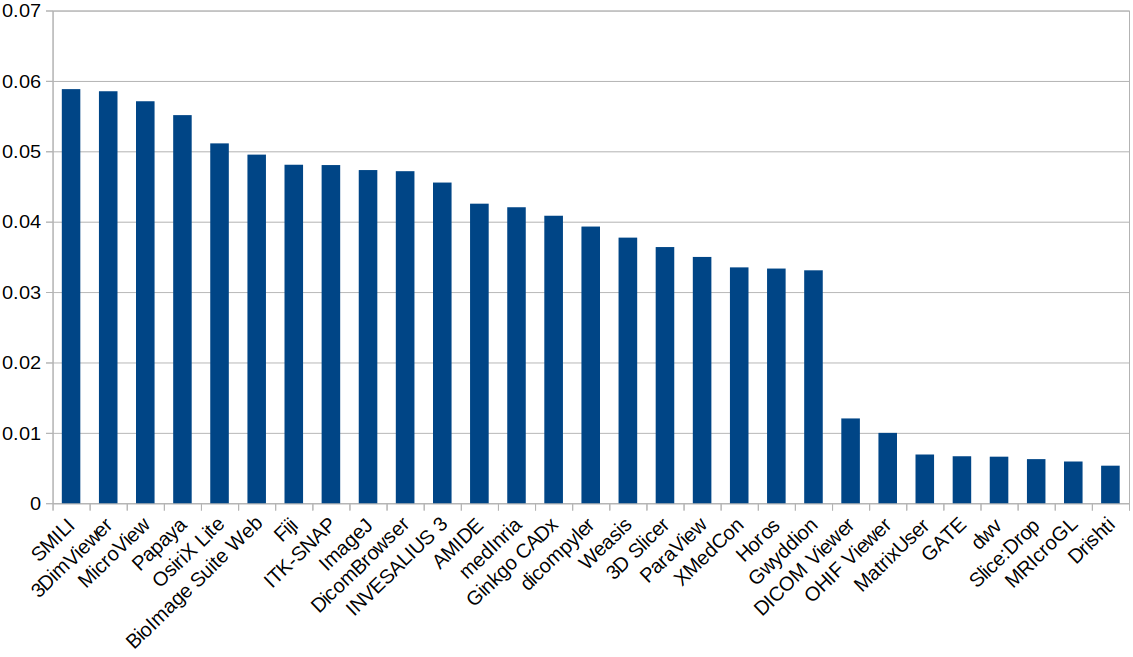
\includegraphics[scale=0.38]{figures/robustness_scores.png}
\caption{AHP surface robustness scores}
\label{fg_robustness_scores}
\end{figure}

The packages with higher scores elegantly handled the unexpected/unanticipated inputs, normally by showing a clear error message. Again, we could not test \textit{DICOM Viewer}. We also might underestimate the score of \textit{OHIF Viewer} \cite{Ziegler2020} since we needed further customization to load data and the test was not complete. \textit{MatrixUser} \cite{Liu2016}, \textit{dwv} \cite{Martelli2021}, \textit{Slice:Drop} \cite{Haehn2013}, and \textit{MRIcroGL} \cite{Rorden2021} ignored the incorrect format of the input files, and displayed blank or meaningless images. \textit{Drishti} successfully detected the unexpected/unanticipated inputs, but the software crashed as a result. For unknown reasons, \textit{GATE} failed to load both correct and incorrect inputs.

\section{Surface Usability}
We measured \textit{Surface Usability} by examining the documents of the projects and considered software with a getting started tutorial and a user manual easier to use. Meanwhile, we checked if users had any channels to get supports. Our impressions and user experiences when testing the software also affected the scores a lot. For example, easy-to-use graphical user interfaces gave us better experiences.

Figure \ref{fg_usability_scores} lists the AHP scores for all packages. The ones with higher scores usually provided both comprehensive document guidance and a good user experience. \textit{INVESALIUS 3} \cite{Amorim2015} set an good example of detailed and clear user manual. \textit{GATE} also provided a large number of documents, but we think that they conveyed the ideas poorly, so we had trouble understand and use them.

\begin{figure}[H]
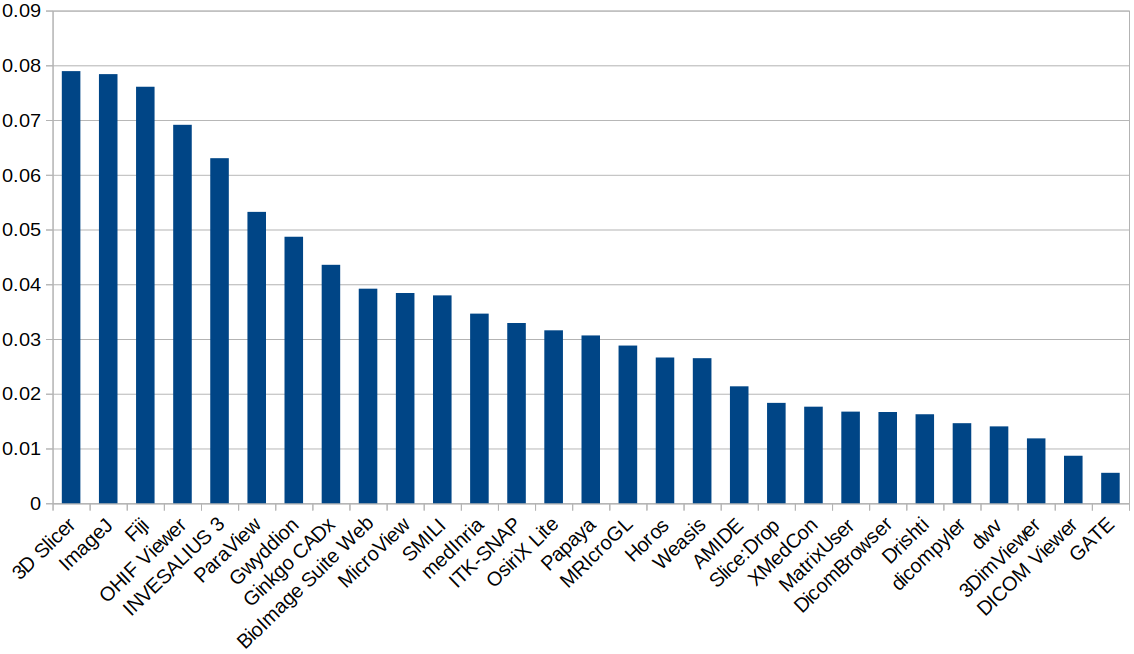
\includegraphics[scale=0.38]{figures/usability_scores.png}
\caption{AHP surface usability scores}
\label{fg_usability_scores}
\end{figure}

\section{Maintainability}

Regarding \textit{maintainability}, we tried to search the projects' documents and identify the process of contributing and reviewing code. We believe that the artifacts of a project - including source code, documents, building scripts, etc. - can significantly affect its  \textit{maintainability}. Thus we checked each project for its artifacts, such as API documentation, bug tracker, release notes, test cases, build files, version control, etc. We also checked which tools supported issue tracking and version control and the percentages of closed issues and comment lines in code. Figure \ref{fg_maintainability_scores} shows the AHP results for \textit{maintainability}. 

\begin{figure}[H]
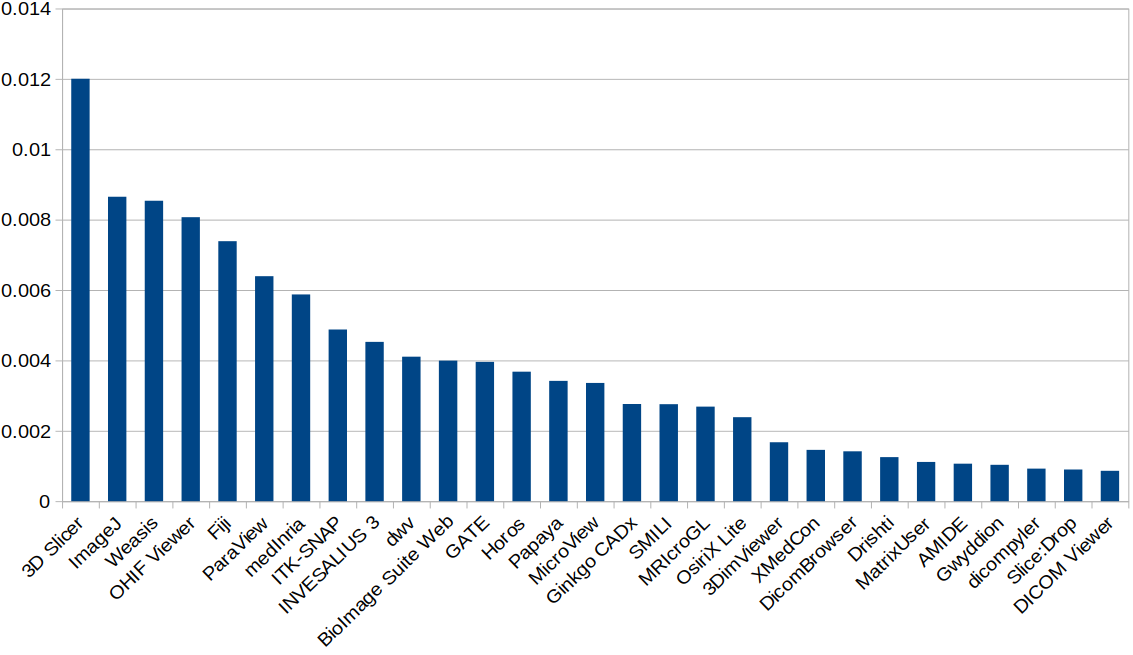
\includegraphics[scale=0.38]{figures/maintainability_scores.png}
\caption{AHP maintainability scores}
\label{fg_maintainability_scores}
\end{figure}

We marked \textit{3D Slicer} with a much higher score than others because it did very well at closing the identified issues, and more importantly, we found it to have the most comprehensive artifacts. For example, as far as we could find out, only 5 out of the 29 projects had a project plan, 6 of them had a developer's manual, and 7 with API documentation, and \textit{3D Slicer} included all these documents.

\section{Reusability}

To measure \textit{reusability}, we counted the total number of code files for each project. We considered the projects with more code files to be more reusable. As mentioned in Section \ref{sec_empirical_measurements}, the tools \textit{GitStats} and \textit{scc} count this number with minor differences, and we used the result from \textit{GitStats} for all projects. We also decided that the projects with API documentation can deliver better \textit{Reusability}. The AHP results are in Figure \ref{fg_reusability_scores}.

\begin{figure}[H]
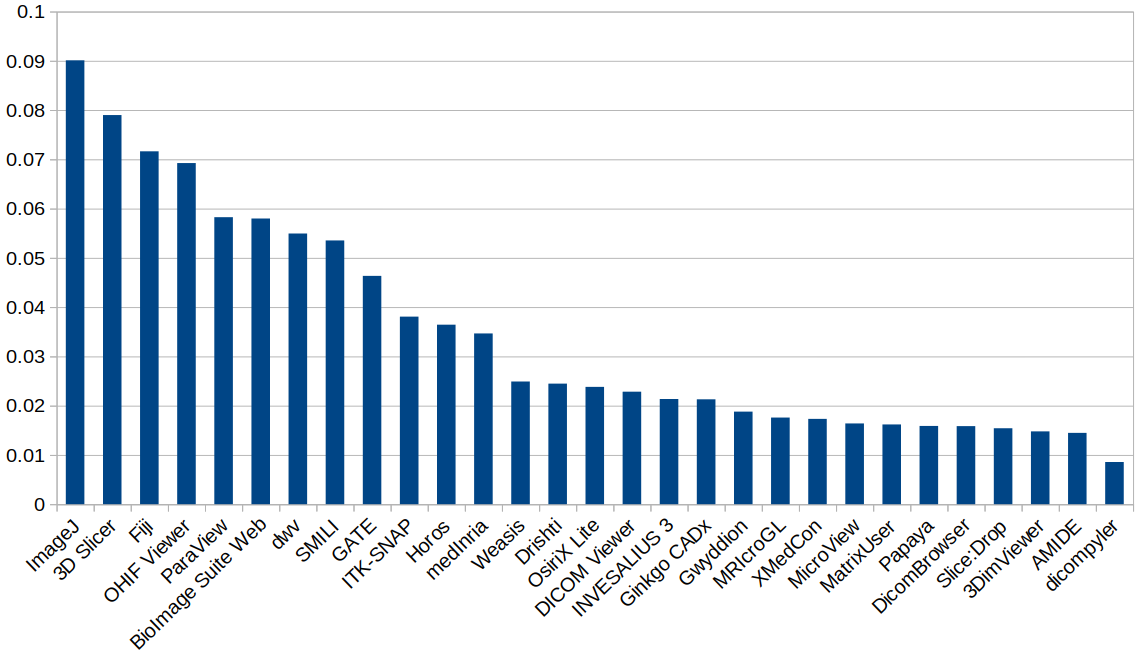
\includegraphics[scale=0.38]{figures/reusability_scores.png}
\caption{AHP reusability scores}
\label{fg_reusability_scores}
\end{figure}

\section{Surface Understandability}

To determine the \textit{surface understandability} for each project, we randomly examined 10 code files. We checked the code’s style within each code file, such as whether the identifiers, parameters, indentation, and formatting were consistent, whether the constants (other than 0 and 1) were hardcoded into the code if the developers modularized the code. We also checked the descriptive information for the code, such as documents mentioning the coding standard, the comments in the code, and the descriptions or links for algorithms used in the code. Figure \ref{fg_surface_understandability_scores} shows the scores.

\begin{figure}[H]
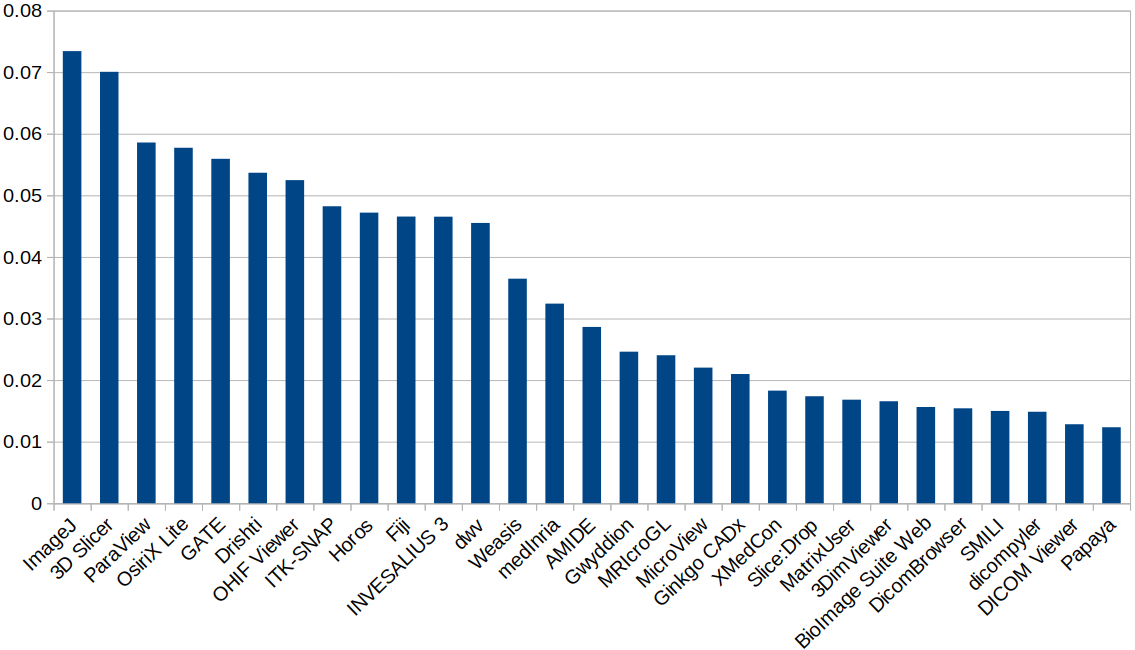
\includegraphics[scale=0.38]{figures/understandability_scores.png}
\caption{AHP surface understandability scores}
\label{fg_surface_understandability_scores}
\end{figure}

Most projects had a consistent style for the code, but we only found explicit identification of a coding standard for only 3 out of the 29, which are \textit{3D Slicer}, \textit{Weasis} \cite{Roduit2021}, and \textit{ImageJ}.

\section{Visibility/Transparency}

To understand the \textit{visibility/transparency}, such as all of the steps of a software development process and the current status described in Section \ref{sec_software_quality}, we tried to access this information from the existing documents. We tried to examine the development process, current status, development environment, and release notes for each project. If any information was missing or poorly conveyed, the \textit{visibility/transparency} was not ideal.

Figure \ref{fg_visibility_transparency_scores} shows the AHP scores. Generally speaking, the teams that actively documented their development process and plans scored higher because they delivered better communication to people outside the team.

\begin{figure}[H]
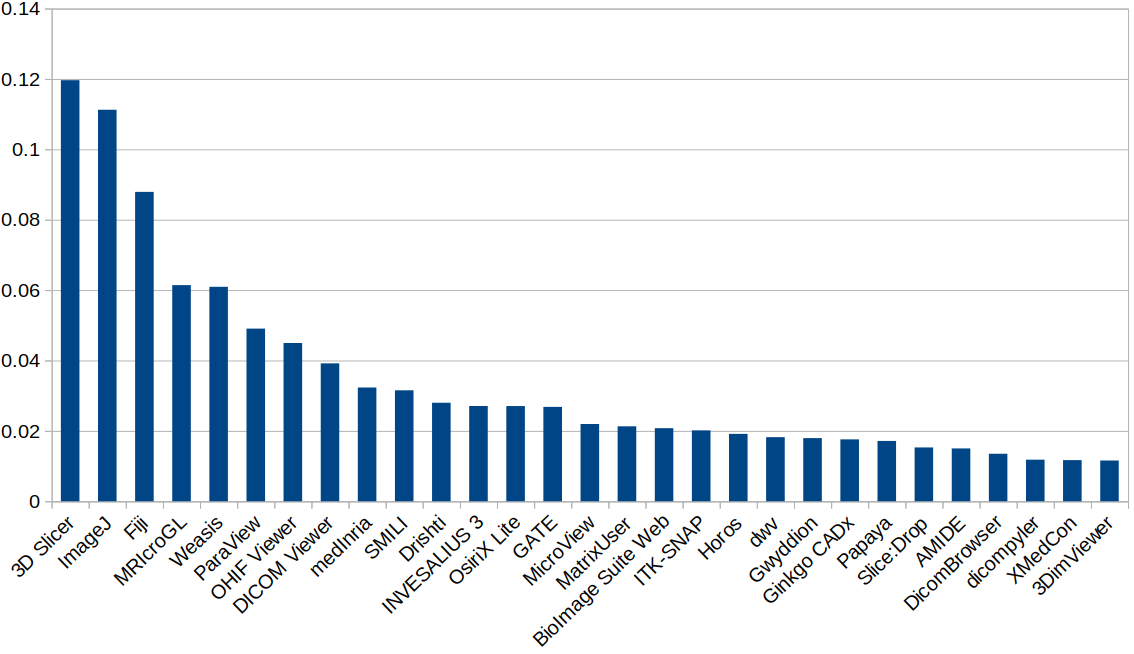
\includegraphics[scale=0.38]{figures/visibility_transparency_scores.png}
\caption{AHP visibility/transparency scores}
\label{fg_visibility_transparency_scores}
\end{figure}
